% We propose our {\ourarchabbr} architecture for adaptable block tuning and pruning while training transformer-based {\lmabbr}s. Based on this architecture, we use Fisher information as the scoring function for block tuning and pruning with self-distillation objectives for efficient and accurate training. Meanwhile, we develop our parameter scheduler that controls the training process, which would gradually discard non-salient parameters during the training stage and re-allocate the tuning parameters in {\ourarchabbr}s, given an overall budget for tuning parameters. Based on these techniques, we can prune out a smaller task-specific model with high training and inference efficiency.

% Around the research question above, we claim three important factors towards better efficient tuning and pruning:

% \noindent $\bullet$ \textbf{Tuning Adaptivity (TA)}: the capability of identifying salient blocks in the {\lmabbr} to be tuned, especially when the convergence speed of PEFT methods is slower than fully fine-tuning, the selection of tuning blocks plays an essential role in model's performance;

% \noindent $\bullet$ \textbf{Pruning Adaptivity (PA)}: considering block-wise information such as uniqueness~\citep{santacroce_what_2023} instead of pruning with salience metrics only. It is especially crucial to the pruned model's performance in PEFT models since the budget for tuning parameters is limited;

% \noindent $\bullet$ \textbf{Distillation Adaptivity (DA)}: the distillation objectives should be able to recover the performance loss layer-wise. Specifically, when a whole transformer layer is pruned at the end, it is critical to find a capable student layer to recover its knowledge.

\section{Problem Formulation} \label{sec:formulation}
% \qq{need to clarify the masks, used for pruning or tuning? what are their purposes, seems they are to decide which parameters to prune or tune based on the description next, then make it clear here.}
% \todo{Make the formulation general and also discuss existing methods' solutions. The problem should be maintaining the performance to some extent, but minimizing the training and inference efficiency. Our solution is more comprehensive considering training and inference.}
% \hanna{you should define the input with notations, then show the equation. It is not feasible to understand this equation without looking at what comes next. Our goal is learn the model m, with parameters theta, ... what is delta; what is gamma.. when you just refer things after explaining the equation is hard. Important things need to be defined first, then equation, then where... here are the parameters.  }

Our goal is to improve the training and inference efficiency of pretrained {\lmabbr} while maintaining task performance. Intuitively, tuning fewer parameters leads to smaller training memory footprints and shorter time per training step; models with fewer parameters also run faster with less memory footprint during inference but come with task performance degradation. We aim to find the optimal parameters for training and inference without sacrificing task performance. 

We formally define the problem objective as minimizing the task loss $\mathcal{L}$ under the constraint that the total {\lmabbr} parameter size $\Theta$ reaches a target sparsity (defined as the ratio of the number of parameters pruned to the original {\lmabbr}) $\gamma_T$ after $T$ training steps. For each training step $t$, the sparsity of the {\lmabbr} remains above $\gamma_t$ while the number of tuning parameters is below $\Delta_t$. We control the pruning masks $\mathcal{M}_t$ and tuning ranks $\mathcal{R}_t$ to satisfy these constraints. We describe the optimization process as:
\begin{equation}
\label{eq:problem}
    \begin{aligned}
        &\operatorname*{argmin}_{\Theta_T, \mathcal{M}_T} & & \frac{1}{|\mathcal{D}|} \sum_{x, y \in \mathcal{D}}\mathcal{L}(x, y|\Theta_T, \mathcal{M}_T) \\
        & \text{s.t. }
        & & 1 - \frac{\mathcal{C}(\Theta_t, \mathcal{M}_t)}{\mathcal{C}(\Theta_0, \mathcal{M}_0)} \geq \gamma_t, \\
        &&& \delta(\Theta_t, \mathcal{M}_t, \mathcal{R}_t) \leq \Delta_t, \\
        &&& \forall t \in \{0, 1, \ldots, T\}.
    \end{aligned}
\end{equation}
where $x, y$ are inputs and labels sampled from the task dataset $\mathcal{D}$, while $\mathcal{C}$ and $\delta$ denotes total and tuning parameter numbers of the {\lmabbr}, respectively.

% where $\Theta_t =\{\theta_t^k\}_{k=1}^n$ and $\mathcal{M}_t = \{M_t^k\}_{k=1}^n$ are the weights\footnote{For instance, there are 6 linear layers in a BERT's transformer layer, where 4 (query, key, value, output) are in MHA while 2 (up, down) are in FFN.} and pruning masks\footnote{The pruning masks denote whether their corresponding blocks shall be pruned (0) or not (1).} in the {\lmabbr}'s $n$ linear layers
% , $\mathcal{C}$ and $\delta$ indicate the number of total and tuning parameters, and $0 < \gamma_t \le 1$ and $\Delta_t$ denotes the pruning and tuning budget schedule.

Based on \cref{eq:problem}, a higher target sparsity $\gamma_T$ improves inference efficiency with fewer FLOPs and memory usage but sacrifices performance. Increasing $\gamma_t$ when $t \ll T$ also improves training efficiency. Besides, tuning more parameters with larger $\Delta$ costs more training memory but makes the model converge faster with better task performance. Our formulation supports task performance improvements together with training and inference efficiency by dynamically adjusting the LM parameters during fine-tuning. 
%Overall, the challenge is balancing training and inference efficiency with model performance.

% as mentioned above, In contrast, {\ourmethod} prunes {\lmabbr}s with $\Delta_t \ll \mathcal{C}(\Theta_t, \mathcal{M}_t)$ by leveraging PEFT methods thus significantly reducing training costs. 

% To vastly prune parameters at the start, we use the cubic sparsity scheduling $\gamma^{(t)} = \gamma^{(T)} + (1-\gamma^{(T)}) (1 - \frac{t-t_0}{T-t_0})^3$ and linearly increase the tuning parameter to control memory and aid performance. 
% \qq{we also need to discuss the tradeoffs (accuracy vs. efficiency, training speed vs. training memory, etc.), your formulation does not show tradeoffs explicitly. Readers can see if you prune too much the efficiency will be higher, but the performance drops, then the first key question is to show the design space, and then your solution described next is the contribution that provides the best tradeoffs.  } \qq{why you are using the schedule? why is it useful here}
% Towards a decent tradeoff between these factors, we use the cubic sparsity scheduling where $\gamma^{(t)} = \gamma + (1-\gamma) (1 - \frac{t-t_0}{T-t_0})^3$ for pruning to vastly discard useless parameters for better efficiency, while we linearly increase the tuning parameter number to avoid notable memory overhead but also benefits the performance recovery.

% Like prior structured pruning methods, we assign a continuous mask ranging from 0 to 1 for each potential pruning block, where the tuning objective is to jointly optimize the model's parameters $\Theta$ together with these masks $M$. Unlike existing methods that set masks as tunable parameters that result in memory overhead in fine-tuning, we only collect corresponding salience scores for every target structure in the {\lmabbr} for optimizing masks. Furthermore, we adjust the continuous masks step-by-step based on those scores for training stability, instead of setting them directly from ones to zeros like post-training pruning settings.

% \begin{figure}[htbp]
%     \centering
%     \includegraphics[width=\columnwidth]{figures/schedule.pdf}
%     \caption{The pruning and tuning schedule in {\ourmethod} compared to fine-pruning and post-training pruning.\hanna{figure is good; the message is not accurately mentioned;  maybe combine with figure 2; figure2 is really complex; and use the same terminology you used in the paper. }}
%     \label{fig:schedule}
% \end{figure}

\section{Adaptive Pruning and Tuning}

\begin{figure*}[t!]
    \centering
    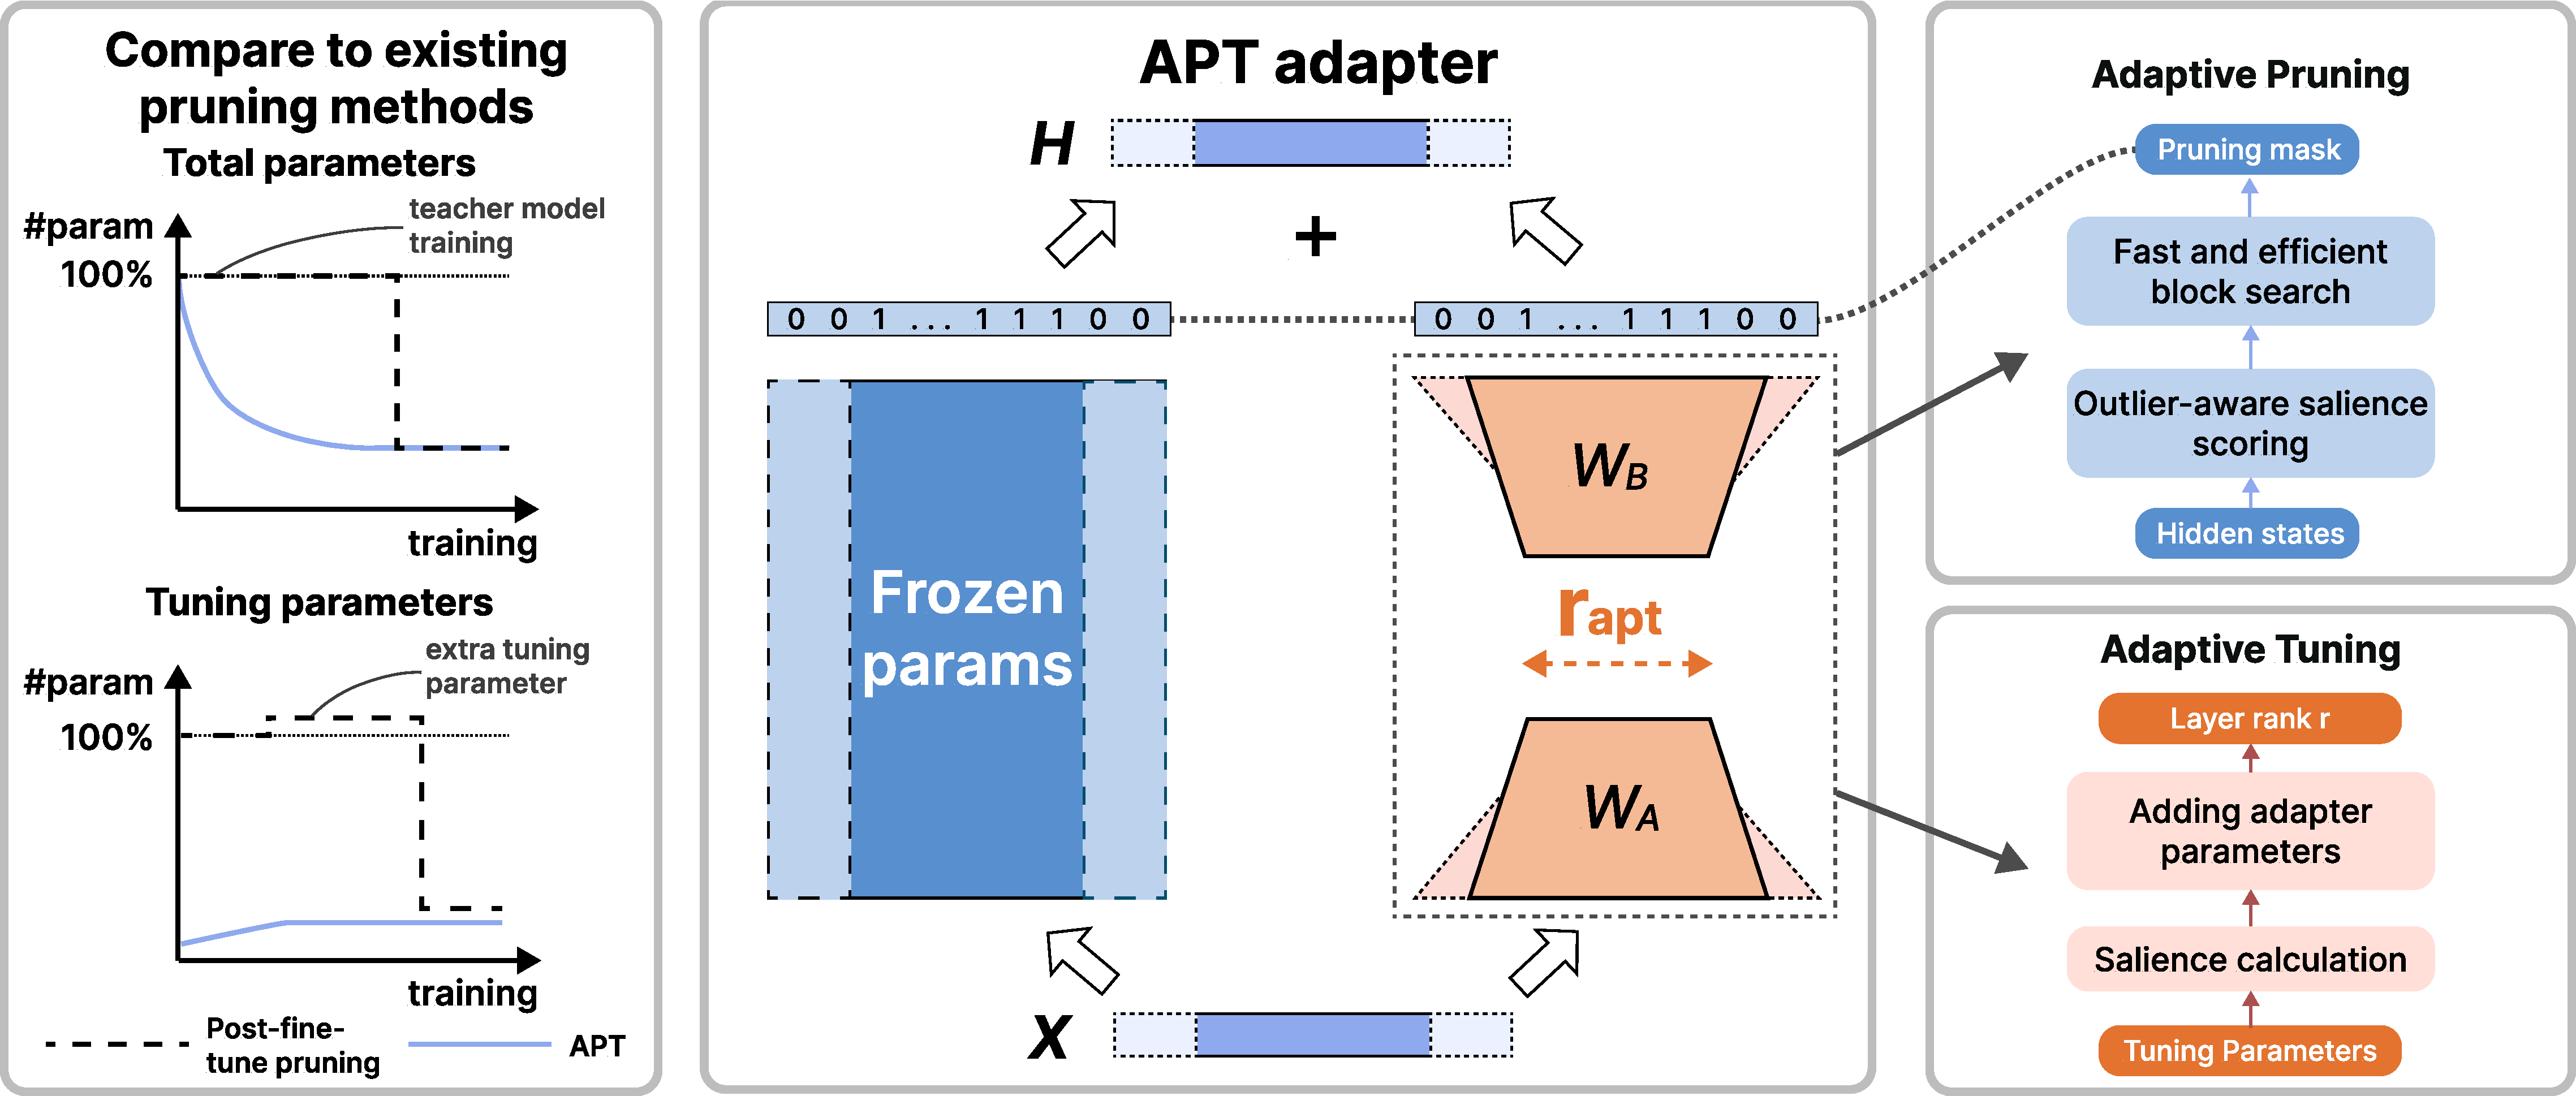
\includegraphics[width=0.95\textwidth]{figures/APT_arch.pdf}
    \caption{{\ourmethod} adaptively identifies pruning and tuning parameters via {\ourarchabbr}s during fine-tuning with little cost. {\ourmethod} gradually prunes {\lmabbr} parameters with binary pruning masks learned from our lightweight outlier-aware salience scoring function for training and inference efficiency. {\ourmethod} also adds tuning parameters in salient layers in {\lmabbr} fine-tuning through increasing dynamic ranks in {\ourarchabbr}s for performance recovery.}
    \label{fig:elastic-adapter}
\vspace{-15pt}
\end{figure*}

We design \textbf{A}daptive \textbf{P}runing and \textbf{T}uning (\textbf{APT}) over {\lmabbr} parameters to allow efficient training and inference while maintaining task performance. 

Summarized in the left of \cref{fig:elastic-adapter}, existing pruning methods often neglect training costs where the number of tuning parameters is more than a parameter-efficient threshold with $\Delta_t \ge \mathcal{C}(\Theta_t, \mathcal{M}_t)$, resulting in long training time and high memory consumption. Instead, to improve training efficiency, we prune {\lmabbr} parameters (increase $\gamma_t$) during early training when $t \ll T$ while keeping $\Delta_t \ll \mathcal{C}(\Theta_t, \mathcal{M}_t)$ to reduce training costs. In addition, we add tuning parameters (increase $\Delta_t$) in early training to effectively mitigate the degradation of {\lmabbr}'s performance due to pruning.

% \subsection{Overview}

% \subsection{{\ourmethod} Overview}
% Some sentences will be moved to the Background section

\noindent \textbf{Overview.} \cref{fig:elastic-adapter} shows the overview of our method that incorporates our new APT adapter for pruning and tuning. Our intuition is that pruning {\lmabbr}s during early fine-tuning will not hurt their task performance while reducing training and inference costs. Meanwhile, unlike existing adapters like LoRA~\cite{hu_lora_2021} that use fixed tuning parameters, APT adapters dynamically add tuning parameters to accelerate {\lmabbr} convergence with superior task performance. We first introduce the architecture of APT adapters in \cref{sec:apt}. We then describe how we prune {\lmabbr} parameters at early fine-tuning with low cost in \cref{sec:apt-prune} and adaptively tune LMs to recover task performance efficiently in \cref{sec:apt-tune}. Additionally, we explain our self-knowledge distillation technique that improves pruned {\lmabbr}'s task performance with limited training expense in \cref{sec:momentum}. 
% during {\lmabbr} fine-tuning, we learn the binary pruning masks via a lightweight outlier-aware salience function with little training cost overhead, and we only add parameters in the top-salient tuning adapters to accelerate convergence with low memory cost.
% \hanna{this is too detailed for an overview; also it has redundancies compared to the opening paragraph, and then lacks motivation why you prune early... Here, just explain the intuition (explained in the intro), then introduce steps according to sub-sections. }
% \hanna{Also, bring  your intuition here -- explained in the intro. }
% \begin{figure}[htbp]
%     \centering
%     \includegraphics[width=\columnwidth]{figures/plot_preliminary_scatter.pdf}
%     \caption{
%     % \hanna{this figure should not be here; maybe it can be moved to the method section or some overview section and only refer to it here}
%     Preliminary study with pruning RoBERTa model on SST-2, where using LoRA with pruning causes large performance degradation while consuming high training time and memory, where {\ourmethod} reaches superior performance and training efficiency.}
%     \label{fig:preliminary}
% \end{figure}

\subsection{{\ourarchabbr}} \label{sec:apt}
We build the {\ourarchabbr} architecture over LoRA, but the key difference is that {\ourarchabbr} supports dynamic {\lmabbr} pruning and tuning. Assuming an {\ourarchabbr} projects the input $X \in \mathbb{R}^{d_i}$ to the output $H_{\text{apt}}(X) \in \mathbb{R}^{d_o}$, we design binary pruning masks ($m_i \in \mathbb{R}^{d_i}$ for input and $m_o \in \mathbb{R}^{d_o}$ for output) and dynamic ranks $r_{\text{apt}}$ in {\ourarchabbr} to control the total and tuning {\lmabbr} parameters during fine-tuning, respectively. Specifically, with tuning parameters $W_A \in \mathbb{R}^{r_{\text{apt}} \times d_i}$ and $W_B \in \mathbb{R}^{d_o \times r_{\text{apt}}}$, {\ourarchabbr} $H_{\text{apt}}$ is denoted as:
\begin{equation} \label{eq:elastic-lora}
        H_{\text{apt}}(X) = m_o \circ (W + s \cdot W_B W_A )X \circ m_i
\end{equation}
where $s$ is the constant scaling factor following LoRA's implementation, and $\circ$ denotes the Hadamard product between the masks and their corresponding matrices. The parameter block is pruned when the multiplying mask is set to 0 and retained when set to 1. In the meantime, during fine-tuning, we dynamically increase $r_{\text{apt}}$ for the weight matrices $W_B$ and $W_A$. Compared to LoRA, APT adapters can be more efficient due to more adaptive pruning and tuning over LM parameters.

In transformer-based {\lmabbr} fine-tuning, we add {\ourarchabbr}s in queries and values of multi-head attention (MHA) layers. We also add {\ourarchabbr} in feed-forward network (FFN) layers when fine-tuning smaller models like RoBERTa and T5 for fast training convergence. In these cases, $m_i$ prunes transformers' hidden dimension and $m_o$ prunes attention heads in MHA and internal neurons in FFN layers. By learning the pruning masks and adjusting the ranks dynamically in the APT adapter, we can achieve the goal defined in \cref{sec:formulation} where the tuning parameter number $\delta(\Theta_t, \mathcal{M}_t, \mathcal{R}_t)$ increases to maintain task performance and the {\lmabbr} parameter size $\mathcal{C}(\Theta_t, \mathcal{M}_t)$ decreases to support more efficient training and inference. Next, we describe the adaptive pruning and tuning procedures in detail.

% Following the notation in \cref{eq: task-formulation}, we can denote {\ourarchabbr} as the layer $\mathcal{E}^k = \{\theta^k, m^k\}$ with the parameter groups $\theta^k = \{W^k, W_B^k,W_A^k, b^k\}$ and masks $M^k=\{m_p^k, m_r^k, m_h^k\}$.


% Based on the {\ourarchabbr} architecture that supports adaptive pruning and tuning, we introduce our Lightweight Parameter Adjustment algorithm to calculate the parameters' salience (weight-gradient production as the importance score) thus identifying and adjusting parameters to be pruned and tuned consuming limited memory. 
% We first introduce how we calculate the approximated parameter salience with outlier awareness, even for those not being tuned, causing limited memory overhead. Afterward, we present our fast knapsack-searching algorithm for transformer pruning. Finally, by combining the parameter pruning and injecting, we show that our Lightweight Parameter Adjustment algorithm can vastly prune a {\lmabbr} with limited resources.

% \begin{equation} \label{eq:sensitivity}
%     \begin{split}
%         % S(W_{i,j}) &= \sum_{(x, y) \in \mathcal{D}} s(W_{i,j}, x, y) \\
%         % &= \sum_{(x, y) \in \mathcal{D}}|\frac{\partial \mathcal{L}(x, y | \Theta)}{\partial W_{i,j}} \cdot W_{i,j}| \\
%         S(W_{:,j}) &= \sum_{(x, y) \in \mathcal{D}}\sum_{i}|\frac{\partial \mathcal{L}(x, y | \Theta)}{\partial W_{i,j}} \cdot W_{i,j}| \\
%         &= \sum_{(x, y) \in \mathcal{D}} (\sum_{i}|\frac{\partial \mathcal{L}(x, y | \Theta)}{\partial X_{j, i}} \cdot X_{j, i}|)
%     \end{split}
% \end{equation}

% \begin{equation} \label{eq:sensitivity}
%     S(m) = |\frac{\partial \mathcal{L}}{\partial m} \cdot m| = \sum_{(X, y) \in \mathcal{D}} |\frac{\partial \mathcal{L}}{\partial H(X)} \cdot H(X)|
% \end{equation}
\subsection{Low-cost Adaptive {\lmabbr} Pruning ($\mathcal{A}_{\text{P}}$)} \label{sec:apt-prune}

% \hanna{this section has some redundancies to previou ssections; it also has too much details that I couldn't follow. Importantly, it is not clear what are novel, what is taken from previous work. }
To benefit the efficiency of LM training and inference, {\ourmethod} adaptively prunes LM parameters since the start of fine-tuning. The problem is finding the parameters to be pruned and discarding them without hurting training stability. Given a task, we compute the outlier-aware salience score of parameter blocks at each early-training step when $t \ll T$. Afterward, we use a fast search algorithm to determine the parameters to be pruned, and then we update their binary pruning masks accordingly. The upper-right of \cref{fig:elastic-adapter} shows this adaptive pruning procedure.

% \hanna{you use the name of outlier-aware salience scoring quite often. Do you introduce this term, or does this exist? instead, you may say we compute a score to obatin saliency of parameters toward an end-task performance? }
% \qq{should describe that pruning happens in two steps, first what metric to decide parameters importance, then do actually pruning, your fast search...}

% \hanna{the following parags can be summarized and made more clear and intuitive; some detailed comments: }
\noindent \textbf{Outlier-aware salience scoring of {\lmabbr} parameters.}
% \qq{for what salience? make it clear, something like ``deciding pruning and tuning parameters" might be better} \bowen{Edited, and I also think the following two sub-subsections shall be compressed later. Or shall they be merged into one?}
When determining the influence of pruning parameters on the {\lmabbr} performance for fine-tuning tasks, the key idea is to compute the outlier-aware salience scores of {\lmabbr} activations to consider both tuning and frozen parameters. 
% \hanna{this sentence about previous work is distracting; maybe move to footnote?}
In detail, salience is defined as the magnitude of parameters' weight-gradient production from previous works~\citep{sanh_movement_2020}, where
\begin{equation} \label{eq:salience}
    S(W_{i, j}) = |{W}_{i,j} \cdot \frac{\partial \mathcal{L}}{\partial {W}_{i,j}}|
\end{equation}

However, since the frozen weights' gradients are unreachable in PEFT settings, we compute the salience as the magnitude of the product of activations and their gradients.
% \hanna{why this product is a representation of a saliency?} \hanna{this next sentence of compression can be moved ot training details.} 
Additionally, we compress the activation and gradients by summing along batches before production to further reduce the training memory consumption. 
% \hanna{don't understand this sentence... have previous work used this? if yes, are you doing exactly the same as previous work, if yes explain it on top}
On the other hand, block outlier parameters play a crucial role in task-specific capabilities, as previous quantization methods suggest~\citep{Dettmers2022LLMint88M,lin2023awq}. Such effects brought by outlier parameters will be averaged if salience is only measured on the block level. To keep more outlier parameters in the pruned {\lmabbr}s, we combine the salience score above and the kurtosis\footnote{Representing the density of the outlier in a distribution, the more the outliers are, the bigger the kurtosis will be.} of the activation together. Therefore, given the supervised finetuning dataset $\mathcal{D}_{t}$, the outlier-aware salience score $\hat{S}$ is defined as:
% \hanna{where did this come from? again ,have other people done it before as well?}
\begin{align}
    % \textrm{Kurt}(X) &= \sum_{(x, y) \in \mathcal{D}} (\sum_i (\frac{X_i - \mu(X)}{\sigma(X)})^4 - 3) \label{eq:kurtosis} \\
    \begin{split}        
        \widetilde{S}_t(W_{:,j}) &= \sum_{(x, y) \in \mathcal{D}_t} \sum_{i} |\frac{\partial \mathcal{L}(x, y | \Theta_t, \mathcal{M}_t)}{\partial H_{j, i}}| \cdot \\
            &\quad \sum_{(x, y) \in \mathcal{D}_t} \sum_{i} | H_{j, i}|
    \end{split} \label{eq:salience-approx} \\
    \hat{S}((W_{:,j}) &= \widetilde{S}(W_{:,j}) + (\textrm{Kurt}(O_{j,:}))^{\frac12} \label{eq:outlier-awared-salience}
\end{align}
where $H$ is the activations in the {\lmabbr}, $\text{Kurt}(\cdot)$ stands for kurtosis, and $O_{:, j} = W_{:, j} \circ X_{j, :}^\intercal$ represents the activation. We leave details of the salience scoring in \cref{appendix:salience-unify}.
% \qq{need to put eq3,4 and 5 together. describe them in one place. First introduce the idea of salience scores, then when describing the details also need to describe why you need them activation instead of parameters, why outlier-aware.}


\noindent \textbf{Efficient search of {\lmabbr} block parameters.}
Given the salience calculated in \cref{eq:outlier-awared-salience}, the next step is to learn the binary pruning masks to increase the {\lmabbr} sparsity above $\gamma_t$. Intuitively, we shall prune the blocks with less salience score, which formulates a latency-saliency knapsack~\citep{NEURIPS2022_5434be94} task.
% To effectively reach the target sparsity, we aim to prune MHA heads, FFN neurons, and the model hidden dimension in transformer-based {\lmabbr}s simultaneously. 
For an {\lmabbr} with $n_L$ transformer layers, where layer $i$ has $n_h^i$ MHA heads and $n_f^i$ FFN neurons, and all transformer layers' hidden dimension sizes are $d_m$, the approximated\footnote{We ignore the model's layer norm and bias terms since their sizes are small, and we do not count tuning parameters since they can be fully merged after training.} number {\lmabbr} parameter is:
\begin{equation} \label{eq:parameter-constraint}
    \mathcal{C}(\Theta_t; \mathcal{M}_t) \approx d_m \sum_{i=1}^{n_L} (4 n_h^i \cdot d_h + 2 n_f^i)
    % &\approx (4 d_h \cdot \sum_h m^h_p + c_f \sum_f m^f_p) \cdot \sum m_h
\end{equation}
where $d_h$ is the dimension per MHA head. To keep the constraint in \cref{eq:problem}, we prune MHA heads, FFN neurons, and the model hidden dimension simultaneously by reducing $n^i_h, n^i_f$, and $d_m$.
% Based on \cref{eq:parameter-constraint}, to reduce the {\lmabbr} parameter $\mathcal{C}(\Theta_t; \mathcal{M}_t)$, we shall decrease $d_m$, $n_h$, and $n_f$ through pruning the hidden dimension, MHA heads, and FFN neurons. 
% \hanna{it seems yepeat the same thing over and over with different wording. First, explain the intuition, then explain the exact thing that you did; the next few sentences are much more clear and probably the most important things in this section, bring them on top.}
Hence, we first sort the blocks by their salience divided by the parameter number. As the parameter size monotonically increases with block quantity, we use binary search to identify the top salient blocks to be retained given the sparsity constraint $\gamma_t$. 
% \hanna{the next few sentences can also be moved into training datails.
We leave the implementation details in \cref{appendix:binary-search} for simplicity.

\subsection{Adaptive and Efficient LM Tuning ($\mathcal{A}_{\text{T}}$)} \label{sec:apt-tune}
% Low-cost lightweight, or what
% Intuitive overall concept -> detail -> equations
% \qq{need a few sentences to describe how tuning works}
As using PEFT methods to fine-tune pruned {\lmabbr}s causes notable performance decrease (illustrated in \cref{tab:small-model-results} and \cref{tab:ablate-paramalloc}), we aim to dynamically add tuning parameters in {\lmabbr} fine-tuning to improve the model's end-task performance. However, since more tuning parameters will consume extra training time and memory, we want to add parameters in a controlled way, where new parameters are only added to task-sensitive {\ourmethod} adapters. As a result, we can recover pruned {\lmabbr}s' performance with reasonable training costs.
% \todo{why adding parameters: 1. pruned LM performance downgrade; 2. less parameter -> less performance but faster and less memory; 3. efficiency is reasonable, but recovering performance}
% Now we present our procedure of adding tuning parameters in salient {\lmabbr} layers for effective {\lmabbr} performance recovery after pruning as depicted in the lower-right section of \cref{fig:elastic-adapter}. To balance training efficiency and performance, we aim to add parameters in a subset of tuning adapter layers selected based on salience \qq{clarify}. \todo{connect to 4.1 above (APT adapters)}
In detail, we first calculate the salience of each {\ourmethod} adapter to determine their importance. Next, we select the top-half {\ourmethod} adapters after sorting them with salience and add their parameters by increasing their $r_{\text{apt}}$.

\noindent \textbf{Salience scoring of {\ourarchabbr}.}
% \hanna{doesn't section 4.3 explain how you compute LM parameter saliency? just refer to it. you can say Given saliency scores of LM parameters (4.2), we define the layer saliency in APT adapter? ... }
Since gradients of tuning parameters information are available when determining the layer salience, we can first calculate each tuning parameter's salience with \cref{eq:salience}. Then, we define the salience of an APT adapter as the summation of the parameter salience scores in $W_B$, denoted as $\mathcal{I}(H_{\text{apt}}) = \sum_{i, j}S({W_B}_{i, j})$, to represent each tuning {\ourarchabbr}'s importance\footnote{The salience scores calculated using $W_B$ and $W_A$ are equal, so using either of them will get the same result.}. Given the calculated $\mathcal{I}(H_{\text{apt}})$ for each {\ourarchabbr}, we can then decide where to add new tuning parameters to efficiently improve the pruned {\lmabbr}'s task accuracy.

\noindent \textbf{Dynamically adding APT adapter parameters to recover task performance.} 
With the importance of {\ourarchabbr}s $\mathcal{I}(H_{\text{apt}})$ calculated, the next step of adaptive tuning is to add tuning parameters by increasing the salient tuning layers' ranks $r_{\text{apt}} \in \mathcal{R}_t$ following budget $\Delta_t$. Therefore, firstly, we sort all tuning layers according to their importance score $\mathcal{I}(H_{\text{apt}})$ and linearly increase the ranks of the top-half salient ones. More specifically, when increasing the tuning parameter from $\Delta_t$ to $\Delta_{t'}$, the salient layer's rank is changed from $r_{\text{apt}}$ to $r_{\text{apt}}' = \lfloor r_{\text{apt}} \cdot \frac{\Delta_{t'}}{\Delta_t} \rfloor$ where $\lfloor \cdot \rfloor$ denotes the floor operation. For training stability, when adding parameters and converting $W_B \in \mathbb{R}^{d_o \times r_{\text{apt}}}, W_A \in \mathbb{R}^{r_{\text{apt}} \times d_i}$ to $W_B' \in \mathbb{R}^{d_o \times r_{\text{apt}}'}, W_A' \in \mathbb{R}^{r_{\text{apt}}' \times d_i}$, we concatenate random Gaussian initialized parameters $\mathcal{N}(0, \sigma^2)$ in $W_A$ and zeros in $W_B$ same as the LoRA initialization, so the layer's output remains unchanged before and after new parameters added.

% Existing fine-pruning methods cost longer training time because of joint optimization of parameters and masks. To speed up training, we propose our fast-searching method to prune a transformer model's blocks (MHA heads, FFN neurons, and hidden dimensions) purely based on salience scores from \cref{eq:outlier-awared-salience} without extra controlling modules. 



% \qq{you need to provide context why you need to allocate parameters for tuning, is it because the performance drop, or for efficiency tradeoffs, etc.}
% To tackle the performance downgrade challenge, we linearly increase the top-half salient tuning layers' LoRA weights in training. To control memory usage, we also discard stably unimportant parameters at the early stage. As shown in \cref{tab:ablate-paramalloc}, we can see that adjusting the layer's parameter size based on salience always yields better results.

% Furthermore, with the scoring function defined in \cref{eq:salience-approx}, we can conduct pruning before tuning to further reduce the memory consumption as shown in \cref{tab:llama-7b-results}. For the pruning during tuning, 
% Overall, our Lightweight Parameter Adjustment algorithm is summarized as \cref{alg:epa} while the schedule is as depicted in \cref{fig:schedule}.



\subsection{Efficient Self-Knowledge Distillation} \label{sec:momentum}
% \qq{This section can be compressed, too many details, you can start with why the Self-Momentum Distillation is needed, due to accuracy drop? and then how you can improve accuracy w/o extra overhead due to distillation (because naive distillation causes memory overhead, making training inefficient.) Summarize the key techniques you used, briefly describe the key ideas and how they improve performance without overhead} 
As shown in \cref{tab:ablate-paramalloc}, training pruned {\lmabbr} without knowledge distillation causes significant end-task performance drops. Therefore, we use knowledge distillation in {\ourmethod} to recover the pruned {\lmabbr}'s performance. Still, existing strategies require a fully trained teacher model being put into the GPU with the student during distillation, causing high training time and memory. To avoid extra training costs, we keep duplicating the tuning student layers as teachers during fine-tuning to reduce total training time. Meanwhile, frozen parameters are shared between the student and teacher model during training to reduce memory consumption. We edit the distillation objective in CoFi~\citep{xia_structured_2022} as
% Furthermore, after the student model's pruning masks are settled and fixed, we select student layer weights using masks $m_p$ and $m_h$ from the shared weights instead of conducting multiplication in high-sparsity pruning settings for further training memory reduction. 
\begin{equation}
    \begin{split}
        % \mathcal{L} &= \mu (\lambda \mathcal{L}_{pred} + (1 - \lambda) \mathcal{L}_{layer}) + (1 - \mu) \mathcal{L}_{ft} \\
        \mathcal{L} &= \mu \mathcal{L}_{distill} + (1 - \mu) \mathcal{L}_{ft} \\
        \mathcal{L}_{layer} &= \sum_{i=1}^\mathcal{T} \textrm{MSE}(\text{Tr}(H_s^{\phi(i)}), H_t^i)
    \end{split}
\end{equation}
where $\mu$ is a moving term linearly scales from 0 to 1 during distillation to encourage the pre-pruned model vastly fit to the training data, $\mathcal{L}_{distill}$ is the distillation objective from CoFi, and $\mathcal{L}_{ft}$ is the supervised fine-tuning objective. $\mathcal{T}$ is block-wise randomly sampled teacher layers following~\citep{haidar2022rail}, $\phi(\cdot)$ is the teacher-student layer-mapping function that matches the teacher layer to its closest, non-pruned student layer. $\text{Tr}$ denotes the tunable LoRA layer for layer transformation, initialized as an identical matrix $\mathcal{I}$. More implementation details of our self-distillation technique is introduced in \cref{appendix:hyper-param}.

% \noindent \textbf{Dynamic layer mapping for better pruning adaptivity.} As for selecting the teacher layers $\mathcal{T}$ during each training step, we randomly sample $n$ layers from the teacher model since existing research found that this strategy yields better distillation results. However, we find that dynamic teachers combined with the dynamic student selection method from CoFi would result in layer-shifting (only bottom student layers are selected, even though the teacher comes from the top), especially in larger encoder-decoder models like T5. Besides, we find that the advantage of CoFi's distillation mainly comes from the layer mapping when the student layer is entirely pruned. Therefore, for the layer mapping function $\phi(\cdot)$, we will do a static mapping if the corresponding layer is not being pruned in the student model, or otherwise, we would dynamically map it to the most similar neighbor layer in the student model:
% \begin{equation}
% \begin{split}
%   \phi(i) &= \displaystyle\argmin_{j \in n(i)} \text{MSE}(W_{tr} H_s^j, H_t^i)
% \end{split}
% \end{equation}
% where $n(i)$ denotes the preserved neighbor layers of the pruned layer, either on its top or bottom. Empirically, this strategy will always find the most effortless teacher layer for student layers to be learned from without raising any layer-shifting problem. 